\documentclass[12pt,a4paper]{article}
\usepackage{geometry}
\geometry{margin=2.5cm}
\usepackage[utf8]{inputenc}
\usepackage[slovene]{babel}
\usepackage{graphicx}
\usepackage{hyperref}
\usepackage{listings}
\usepackage{xcolor}
\usepackage{setspace}
\usepackage{fancyhdr}
\usepackage{titlesec}
\usepackage{enumitem}

\lstset{
    basicstyle=\ttfamily\small,
    keywordstyle=\color{blue},
    commentstyle=\color{gray},
    stringstyle=\color{red},
    breaklines=true,
    showstringspaces=false,
    frame=single,
    captionpos=b,
    belowcaptionskip=10pt
}

\onehalfspacing
\pagestyle{fancy}
\fancyhf{}
\fancyfoot[C]{\thepage}
\setlength{\parindent}{0pt}
\setlength{\parskip}{0.8em}

\titleformat{\section}{\normalfont\Large\bfseries}{\arabic{section}}{1em}{}
\titleformat{\subsection}{\normalfont\large\bfseries}{\thesection.\arabic{subsection}}{1em}{}
\titleformat{\subsubsection}{\normalfont\normalsize\bfseries}{\thesubsection.\arabic{subsubsection}}{1em}{}

\begin{document}

% Naslovna stran
\begin{titlepage}
    \thispagestyle{empty}
    \begin{center}
        
\includegraphics[width=5cm]{slike/logotip_vegova_leze_brezokvirja.png}

        \vspace{2cm}

        {\Large \textbf{SEMINARSKA NALOGA PRI RAČUNALNIŠTVU}}

        \vspace{1.5cm}

        {\Huge \textbf{SPLETNA APLIKACIJA MEDIFORM ZA DIGITALNO POROČANJE O ZDRAVSTVENI NEGI}}

        \vspace{1.5cm}

        {\large \textbf{Strokovno poročilo}}

        \vfill

        \begin{flushleft}
        Mentor: mag. Aleš Volčini, prof. \hfill Avtor: Lin Čadež, G 4. A
        \end{flushleft}

        \vspace{0.5cm}

        Ljubljana, april 2026
    \end{center}
\end{titlepage}

\section*{Zahvala}

Zahvaljujem se mentorju Alešu Volčiniju za strokovno pomoč, usmerjanje in koristne pripombe pri izdelavi seminarske naloge ter pri razvoju aplikacije MediForm.

Posebna zahvala gre Heleni Božič Janežič s Srednje zdravstvene šole Ljubljana za sodelovanje, pojasnila glede obstoječega načina dela, posredovana gradiva in sprotne povratne informacije. Zahvaljujem se tudi dijakom, ki so aplikacijo preizkušali in s svojimi predlogi pomagali izboljšati uporabniško izkušnjo.

\newpage

\section*{Povzetek}

V tem strokovnem poročilu sem predstavil razvoj spletne aplikacije MediForm, ki sem jo izdelal za Srednjo zdravstveno šolo Ljubljana. Aplikacija je namenjena dijakom zdravstvene nege za sprotno in strukturirano izpolnjevanje poročil o praktičnem pouku. Odločil sem se za digitalno rešitev, ker so bila papirna poročila zamudna, neenotna in pogosto izpolnjena šele tik pred rokom oddaje.

V poročilu sem opisal analizo potreb naročnika, dogovarjanje in komunikacijo s stranko, izbiro tehnologij ter tehnično izvedbo ključnih funkcionalnosti. Ker je končna rešitev zasnovana kot frontend-only aplikacija, podatke shranjujem v piškotke in v lokalno shrambo brskalnika. Tak pristop sem izbral zato, ker je bila aplikacija namenjena preprosti uporabi brez dodatne strežniške infrastrukture, šola pa ima tako večji nadzor nad informacijami in lažje upravlja z objavljeno različico.

Ugotovil sem, da je tesna komunikacija s stranko pomembna za uspešen razvoj in da aplikacija resnično olajša delo uporabnikom.

\textbf{Ključne besede:} spletna aplikacija, MediForm, zdravstvena nega, praktični pouk, React, TypeScript, Tailwind CSS, cookies, localStorage, analiza podatkov

\newpage

\tableofcontents

\newpage

\section{Uvod}

V sodobnem času se šole vse pogosteje srečujejo s potrebo po digitalizaciji administrativnih postopkov. Tudi v zdravstvenem izobraževanju se pojavlja problem, da dijaki poročila o praktičnem pouku pogosto izpolnjujejo prepozno, površno ali neenotno. To zmanjšuje preglednost dela in otežuje sprotno spremljanje opravljenih aktivnosti.

Na podlagi tega konkretnega problema sem se odločil razviti spletno aplikacijo MediForm. Z njo sem želel dijakom omogočiti, da poročila izpolnjujejo sproti, z vnaprej pripravljenimi možnostmi izbire in z manj ročnega tipkanja. Hkrati sem želel narediti rešitev, ki je dovolj pregledna, varna in preprosta za uporabo v šolskem okolju.

Cilji seminarske naloge so bili naslednji:
\begin{itemize}
    \item analizirati potrebe naročnika,
    \item razviti spletno aplikacijo za poročanje o zdravstveni negi,
    \item pojasniti uporabljene tehnologije,
    \item opisati ključne dele kode in razlog za takšno zasnovo,
    \item pokazati, kako je potekalo delo in komunikacija s stranko,
    \item predstaviti rezultate analize uporabe aplikacije.
\end{itemize}

\section{Teoretični uvod}

Digitalna transformacija v izobraževanju pomeni uvajanje digitalnih tehnologij v učne in administrativne procese. Pri strokovnem in poklicnem izobraževanju je ta prehod še posebej pomemben, ker omogoča boljšo preglednost, hitrejše delo in manj napak pri dokumentiranju. Evropska komisija poudarja, da digitalna orodja izboljšujejo dostopnost informacij in omogočajo učinkovitejše upravljanje izobraževalnih procesov (European Commission, 2020).

Pri digitalnih obrazcih je pomembno, da so vnosni postopki enostavni in strukturirani. Selwyn (2016) izpostavlja, da digitalni sistemi zmanjšujejo potrebo po ponavljajočem ročnem zapisovanju in omogočajo bolj dosledno obdelavo podatkov. Tudi razvoj oblačnih rešitev, kot je Firebase, prispeva k večji dostopnosti in prilagodljivosti aplikacij, saj podatki niso vezani na eno napravo ali eno lokacijo (Firebase, 2026).

V MediForm sem zato uporabil načela digitalne preglednosti, varnega shranjevanja podatkov in sprotnega beleženja. Takšen pristop je bil primeren za okolje zdravstvene nege, kjer je pomembno, da dijaki poročila izpolnjujejo redno in v čim bolj enotni obliki.

Pri razvoju spletne aplikacije sem se opiral tudi na osnovna načela spletnih tehnologij. HTML sem uporabil kot strukturo obrazcev, CSS oziroma Tailwind CSS za oblikovanje in preglednost, JavaScript pa za logiko uporabniške interakcije. React mi je omogočil, da sem posamezne dele vmesnika razdelil v komponente in jih lažje ponovno uporabil, TypeScript pa mi je pomagal pri natančnejšem razvoju, ker sem že med pisanjem opazil morebitne napake v tipih.

Za lokalno razvijanje in hitrejše testiranje sem uporabil Vite, ker sem lahko spremembe vmesnika hitro preveril brez dolgotrajnega zaganjanja. To je bilo pomembno predvsem pri delu z več vnosnimi polji, tabelami in izbirnimi seznami, kjer je bilo treba večkrat preveriti, kako se elementi obnašajo na različnih zaslonih. Takšna izbira tehnologij je bila skladna z mojim ciljem, da aplikacijo razvijem pregledno, hitro in dovolj preprosto za šolsko uporabo.

\section{Jedro}

\subsection{Analiza problema in komunikacija s stranko}

\subsubsection{Obstoječi način dela}

Ko sem prvič stopil v stik s Heleno Božič Janežič s Srednje zdravstvene šole Ljubljana, mi je predstavila obstoječi način izpolnjevanja poročil. Dijaki zdravstvene nege so dokumentacijo izpolnjevali na papirju, pogosto tik pred rokom oddaje. Ugotovil sem, da je tak način dela povzročal več težav:

\begin{itemize}
    \item zapisi so bili pogosto površni,
    \item nekateri deli poročil so se ponavljali,
    \item sprotnega preverjanja skoraj ni bilo,
    \item ročno pisanje je bilo za dijake zamudno.
\end{itemize}

\subsubsection{Proces dogovarjanja}

Proces dogovarjanja sem razdelil na več faz. Najprej sem prejel papirne obrazce in skupaj z naročnico pregledal, kateri deli so zares potrebni in kateri bi se lahko poenostavili. Na podlagi tega sem zasnoval prvo verzijo aplikacije.

Ko so dijaki začeli aplikacijo uporabljati, sem dobil prve povratne informacije. Ugotovil sem, da so se pri prijavi pojavile težave, zato sem popravil način shranjevanja stanja in izboljšal stabilnost delovanja. Kasneje je naročnica predlagala, da bi bilo bolje, če bi dijaki večino podatkov le označevali z izborom možnosti, ne pa jih ročno vnašali.

V nadaljevanju sem aplikacijo dopolnjeval glede na pripombe iz prakse. Naročnica je posebej poudarila, da mora biti rešitev primerna za uporabo na telefonu, da mora omogočati sprotno izpolnjevanje in da morajo biti nekateri deli obrazca poenostavljeni. Na tej osnovi sem odstranil odvečne elemente in izboljšal uporabniški vmesnik.

\subsubsection{Ključne ugotovitve}

Iz komunikacije s stranko sem ugotovil naslednje:
\begin{itemize}
    \item večina podatkov se v poročilih ponavlja,
    \item uporabniki potrebujejo hitro in enostavno izpolnjevanje,
    \item aplikacija mora delovati na različnih napravah,
    \item sprotno shranjevanje je nujno,
    \item zasebnost pacientovih podatkov mora biti ustrezno zaščitena.
\end{itemize}

\subsection{Izbira tehnologij}

Pri razvoju sem se odločil za naslednji tehnološki sklad:

\begin{itemize}
    \item \textbf{React} in \textbf{TypeScript} za uporabniški vmesnik,
    \item \textbf{Tailwind CSS} za oblikovanje,
    \item \textbf{Vite} za hiter razvoj in lokalno testiranje,
    \item \textbf{Cookies} in \textbf{localStorage} za shranjevanje stanja v brskalniku.
\end{itemize}

Za ta izbor sem se odločil, ker omogoča hitro razvojno delo, dobro preglednost kode in enostavno nadgradnjo aplikacije. V produkcijski različici sem se odpovedal strežniškemu delu, saj gre za frontend-only rešitev, v kateri želim imeti podatke pod nadzorom znotraj same spletne strani in brskalnika.

Pri primerjavi z lanskimi rešitvami sem posebej pazil, da so tehnološka pojasnila krajša, a bolj povezana z dejanskim delovanjem aplikacije. Namesto splošnega opisa sem se osredotočil na to, kako React, TypeScript in piškotki konkretno pomagajo pri izpolnjevanju obrazca, prikazu podatkov in preprostem objavljanju spletne strani.

\subsection{Arhitektura aplikacije}

Aplikacijo sem zasnoval kot frontend-only rešitev. Vse bistvene funkcionalnosti potekajo v brskalniku, podatke pa shranjujem v piškotke in lokalno shrambo. Takšna zasnova je bila primerna, ker aplikacija ne potrebuje ločenega strežniškega dela in je zato enostavnejša za vzdrževanje, objavo in uporabo v šolskem okolju.

\begin{figure}[h]
    \centering
    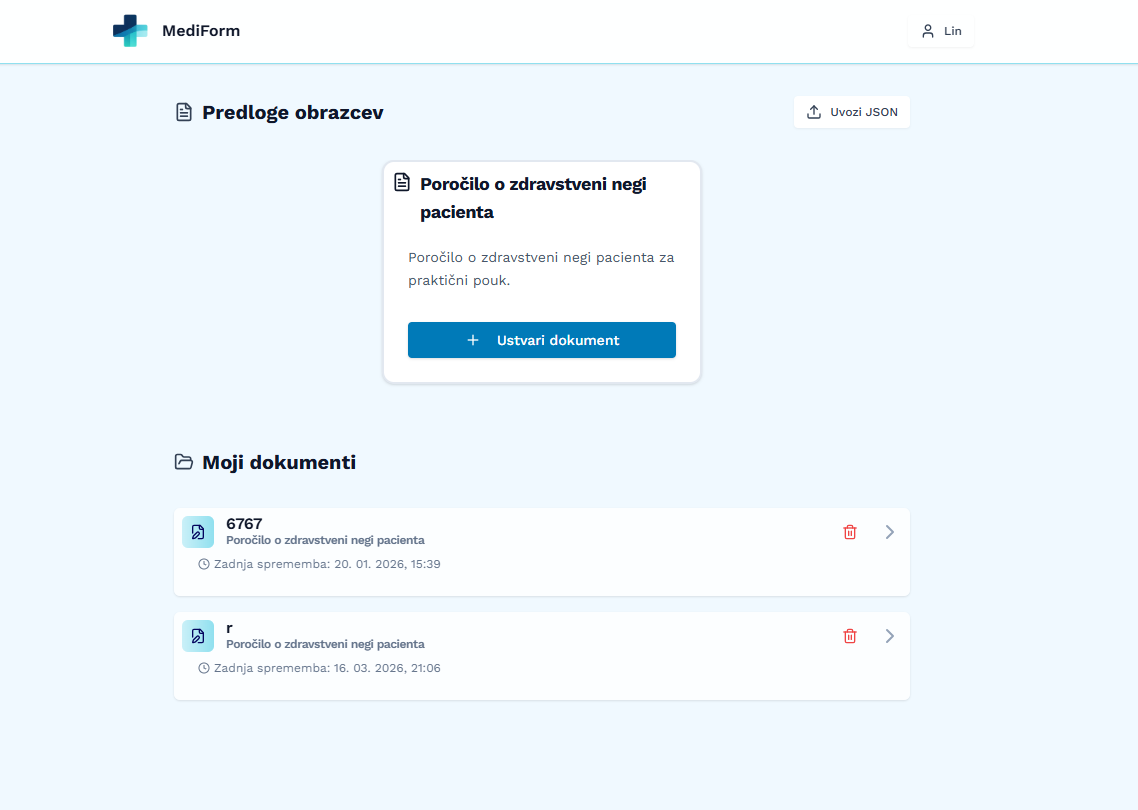
\includegraphics[width=0.8\textwidth]{slike/mediform_user_area_home_page.png}
    \caption{Slika 1: Domača stran aplikacije MediForm}
\end{figure}

Takšna arhitektura omogoča jasno ločitev odgovornosti med prikazom podatkov in njihovim shranjevanjem v brskalniku. Uporabniški vmesnik je pregleden, logika pa ostane v sami aplikaciji, zato je objava hitrejša in enostavnejša.

\subsection{Tehnična izvedba ključnih funkcionalnosti}

\subsubsection{Struktura obrazca in izbira podatkov}

Pri zasnovi obrazca sem se odločil, da bodo ključni podatki prikazani v obliki spustnih seznamov, večkratnih izbir in krajših besedilnih vnosov. Tak pristop sem izbral zato, ker je dijakom na praksi hitrejši od ročnega tipkanja daljših opisov.

\begin{figure}[h]
    \centering
    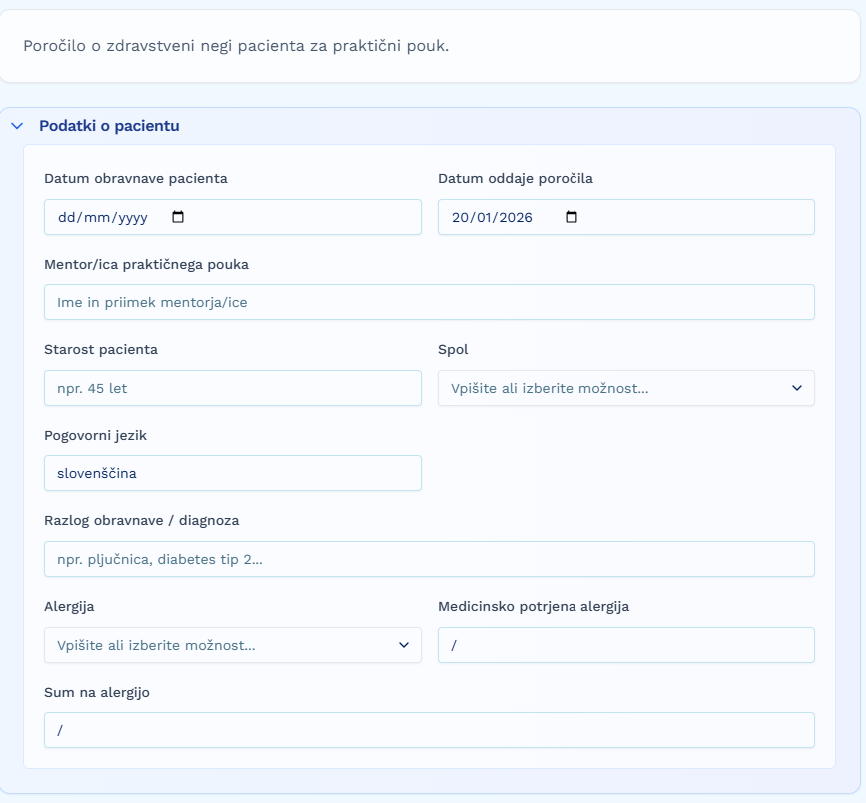
\includegraphics[width=0.7\textwidth]{slike/mediform_obrazec_podatkiopacientuu_dropdown_example.png}
    \caption{Slika 2: Primer spustnega seznama za izbiro podatkov}
\end{figure}

\begin{figure}[h]
    \centering
    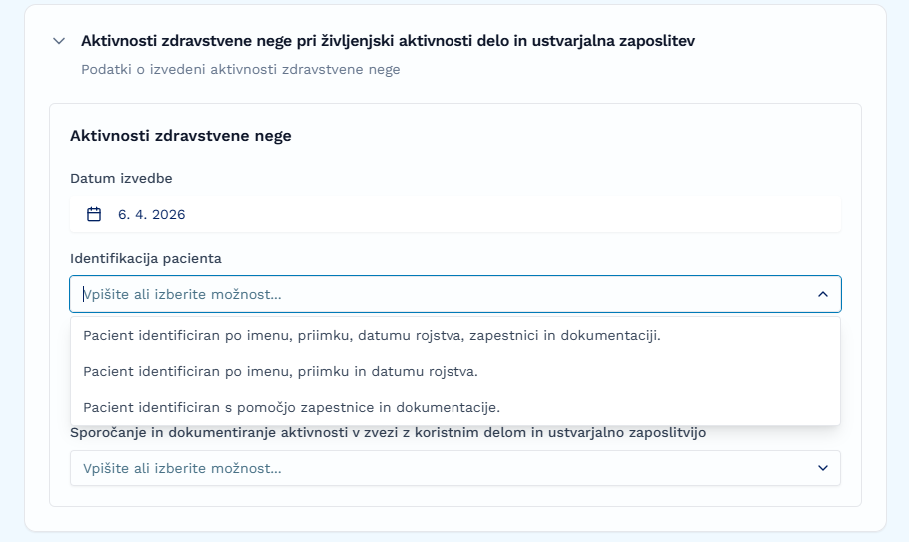
\includegraphics[width=0.7\textwidth]{slike/dropdown_miedform_example_aktivnosti_zdravstvene_nege.png}
    \caption{Slika 3: Primer večkratne izbire aktivnosti zdravstvene nege}
\end{figure}

\textbf{Primer kode --- shranjevanje stanja obrazca v brskalniku:}

\begin{lstlisting}
// Uporaba localStorage za sprotno shranjevanje stanja obrazca
const saveFormState = (formId, formState) => {
  localStorage.setItem(`mediform-${formId}`, JSON.stringify(formState));
};

const loadFormState = (formId) => {
  const storedState = localStorage.getItem(`mediform-${formId}`);
  return storedState ? JSON.parse(storedState) : null;
};
\end{lstlisting}

Razlaga: Funkcija \texttt{saveFormState} ob vsakem pomembnem vnosu shrani celotno stanje obrazca pod enoličnim ključem \texttt{mediform-formId}. Funkcija \texttt{loadFormState} isti ključ prebere ob ponovnem obisku in vrne že izpolnjene vrednosti. V praksi to pomeni, da dijak lahko zapre telefon in nadaljuje kasneje brez ponovnega vnašanja.

\subsubsection{Piškotki in shranjevanje seje}

Namesto strežniške prijave sem uporabil preprost pristop z brskalniškimi piškotki. Ti so primerni za krajše shranjevanje pomembnih nastavitev, ker jih lahko aplikacija prebere ob naslednjem obisku strani.

\textbf{Primer kode --- zapis v piškotek:}

\begin{lstlisting}
// Shrani izbiro uporabnika v piskotek
const setCookie = (name, value, days) => {
  const expires = new Date(Date.now() + days * 86400000).toUTCString();
  document.cookie = `${name}=${encodeURIComponent(value)}; expires=${expires}; path=/; SameSite=Lax`;
};

const getCookie = (name) => {
  const cookies = document.cookie.split('; ').find(row => row.startsWith(`${name}=`));
  return cookies ? decodeURIComponent(cookies.split('=')[1]) : null;
};
\end{lstlisting}

Razlaga: Funkcija \texttt{setCookie} zapiše podatek skupaj z datumom poteka, \texttt{getCookie} pa ta podatek vrne ob naslednjem odprtju aplikacije. Piškotke sem uporabil za manjše podatke (na primer zadnji izbor uporabnika), ker so hitri za branje in ne zahtevajo strežniške infrastrukture.

\subsubsection{Zakaj ni ločenega strežnika}

V zgodnji fazi projekta sem preverjal tudi strežniške možnosti, vendar sem jih v produkcijski različici opustil. Razlog je bil predvsem v tem, da je naročnica želela enostavno rešitev z manj odvisnostmi, šola pa je želela večji nadzor nad informacijami. Zato sem končno različico objavil kot statično spletno stran, kjer so podatki shranjeni lokalno v brskalniku in v piškotkih.

Takšna odločitev je bila smiselna tudi zaradi lažje vzdržljivosti. Če aplikacija ne potrebuje ločenega strežnika, je manj točk, kjer bi lahko prišlo do napake, hkrati pa je objava hitrejša.

\subsubsection{Prikaz napredka obrazca}

Ker mora dijak videti, koliko obrazca je že izpolnil, sem dodal tudi preprost izračun napredka. To je pomembno predvsem zato, ker uporabnik na praksi lažje spremlja, ali je poročilo skoraj končano ali ga mora še dopolniti.

\textbf{Primer kode --- izračun napredka:}

\begin{lstlisting}
const calculateProgress = (completedFields, totalFields) => {
    if (!totalFields) return 0;
    return Math.round((completedFields / totalFields) * 100);
};

const progress = calculateProgress(18, 24);
\end{lstlisting}

Razlaga: V funkcijo podam število izpolnjenih in vseh polj. Rezultat je odstotek, ki ga prikažem v uporabniškem vmesniku. Ta prikaz uporabniku takoj pove, ali je poročilo pripravljeno za oddajo, in zmanjša možnost, da bi spregledal obvezna polja.

\subsubsection{Izvoz v PDF}

Ena od pomembnih funkcij je tudi izvoz poročila v PDF. To je uporabno zato, ker dijak na koncu dobi urejen dokument, ki ga lahko shrani ali predstavi v tiskani obliki.

\textbf{Primer kode --- priprava izvoza v PDF:}

\begin{lstlisting}
const exportToPdf = async (formData) => {
    const pdf = new jsPDF();
    pdf.text('MediForm - porocilo o zdravstveni negi', 14, 15);
    pdf.text(`Ime: ${formData.name}`, 14, 30);
    pdf.text(`Datum: ${formData.date}`, 14, 40);
    pdf.save('mediform-porocilo.pdf');
};
\end{lstlisting}

Razlaga: V funkciji najprej ustvarim nov PDF dokument, nato po vrsticah zapišem ključne podatke obrazca in na koncu datoteko shranim. Prednost takšne izvedbe je, da uporabnik z enim klikom dobi standardizirano poročilo brez ročnega prepisovanja.

\subsubsection{Preverjanje shranjene izbire}

Ko uporabnik ponovno odpre aplikacijo, mu želim prikazati zadnje stanje obrazca. Zato preberem podatke iz brskalnika in jih uporabim za predizpolnitev vmesnika.

\textbf{Primer kode --- branje iz piškotka ali lokalne shrambe:}

\begin{lstlisting}
const getSavedForm = (formId) => {
    const saved = localStorage.getItem(`mediform-${formId}`);
    return saved ? JSON.parse(saved) : {};
};
\end{lstlisting}

Razlaga: Funkcija preveri, ali pod ključem obstaja že shranjen JSON. Če obstaja, ga pretvori nazaj v objekt in ga uporabi za predizpolnitev polj. Če podatka ni, vrne prazen objekt, zato aplikacija deluje stabilno tudi pri prvem obisku.

\subsubsection{Odzivni prikaz na telefonu}

Ker se aplikacija največ uporablja na telefonu, sem moral prilagoditi tudi postavitev elementov. Pri tem sem uporabil odzivne razrede Tailwind CSS, da so gumbi in polja uporabni tudi na manjših zaslonih.

\textbf{Primer kode --- odzivna postavitev:}

\begin{lstlisting}
<div className="grid grid-cols-1 gap-4 md:grid-cols-2">
    <input className="w-full rounded-lg border p-3" />
    <button className="w-full rounded-lg bg-sky-600 p-3 text-white md:w-auto">
        Shrani
    </button>
</div>
\end{lstlisting}

Razlaga: Razreda \texttt{grid-cols-1} in \texttt{md:grid-cols-2} določata, da je na telefonu prikazana ena kolona, na širšem zaslonu pa dve. Gumb je na telefonu čez celo širino, zato je lažje klikljiv med delom na praksi.

\subsubsection{Analiza uporabe aplikacije}

Za preverjanje uporabe sem v razvojni fazi pripravil kratek skript, ki je pregledal lokalno shranjene vnose in iz njih izračunal osnovne statistike. Ta del sem uporabljal samo med testiranjem in ga v produkcijski različici odstrnil, da je šola dobila popoln nadzor nad informacijami ter da v objavljeni aplikaciji ni dodatne analitike, ki bi posegala v zasebnost.

Na podlagi zadnjega izpisa \texttt{backend-usage-dump.json} sem ugotovil, da je aplikacijo uporabljalo 17 uporabnikov, skupaj pa je bilo ustvarjenih 95 poročil, kar pomeni povprečno 5,59 poročila na uporabnika. Iz časovne porazdelitve je razvidno, da se je uporaba pojavljala v tednih W04, W05, W06, W07, W08, W12, W13 in W14, pri čemer je bilo največ aktivnosti v osrednjem delu obdobja, ko je bilo poročanje najbolj intenzivno. Analiza tipov izvoza je pokazala 74 izvozov v PDF in 21 izvozov v JSON, zato je jasno, da je bil PDF v praksi glavna oblika za oddajo poročil.

\section{Git in verzioniranje}

Git sem uporabljal kot glavni mehanizem za nadzor sprememb. Vsako večjo funkcionalnost sem razvil v ločenem sklopu sprememb in jo zaključil z opisnim \texttt{commit} sporočilom. Tako sem lahko natančno sledil, kdaj sem dodal posamezno funkcijo in zakaj sem jo uvedel.

V praksi je to pomenilo:
\begin{itemize}
    \item po vsaki zaključeni funkcionalnosti sem naredil nov commit,
    \item pred večjimi popravki sem primerjal trenutno in prejšnjo različico,
    \item stabilne točke sem označil z oznakami (tag), da sem imel jasno razvojno zgodovino.
\end{itemize}

\textbf{Primer kode --- beleženje verzije v Gitu:}

\begin{lstlisting}
git add .
git commit -m "Dodan izvoz PDF in izboljsan prikaz napredka"
git tag v1.2.0
\end{lstlisting}

Razlaga: Prvi ukaz pripravi datoteke za shranjevanje, drugi ustvari novo verzijo z opisom spremembe, tretji pa označi stabilno izdajo. S tem sem si olajšal testiranje in pripravo objav, ker sem se lahko vedno vrnil na preverjeno stanje.

\section{Deployment (objava aplikacije)}

Deployment sem izvedel kot objavo statične frontend aplikacije. Ker MediForm ne uporablja ločenega strežniškega dela, je bil postopek enostaven: priprava produkcijskega \texttt{build} paketa in objava na domeni \url{https://mediform.cadez.eu/}.

Postopek objave je potekal po korakih:
\begin{enumerate}
    \item lokalno sem preveril, da aplikacija deluje brez napak,
    \item pripravil sem produkcijski build,
    \item objavil sem datoteke na gostovanje,
    \item po objavi sem preveril delovanje obrazca, shranjevanja in izvoza PDF.
\end{enumerate}

Tak pristop je bil primeren za šolsko okolje, ker je objava hitra, stroški so nizki, vzdrževanje pa je preprostejše kot pri aplikaciji z dodatnim strežnikom.

\begin{figure}[h]
    \centering
    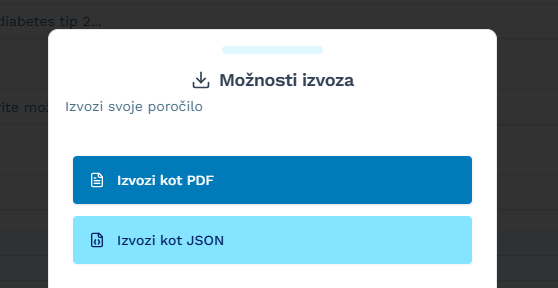
\includegraphics[width=0.8\textwidth]{slike/medifrom_example_moznosti_izvoza_options.png}
    \caption{Slika 4: Primer možnosti izvoza poročila}
\end{figure}

\begin{figure}[h]
    \centering
    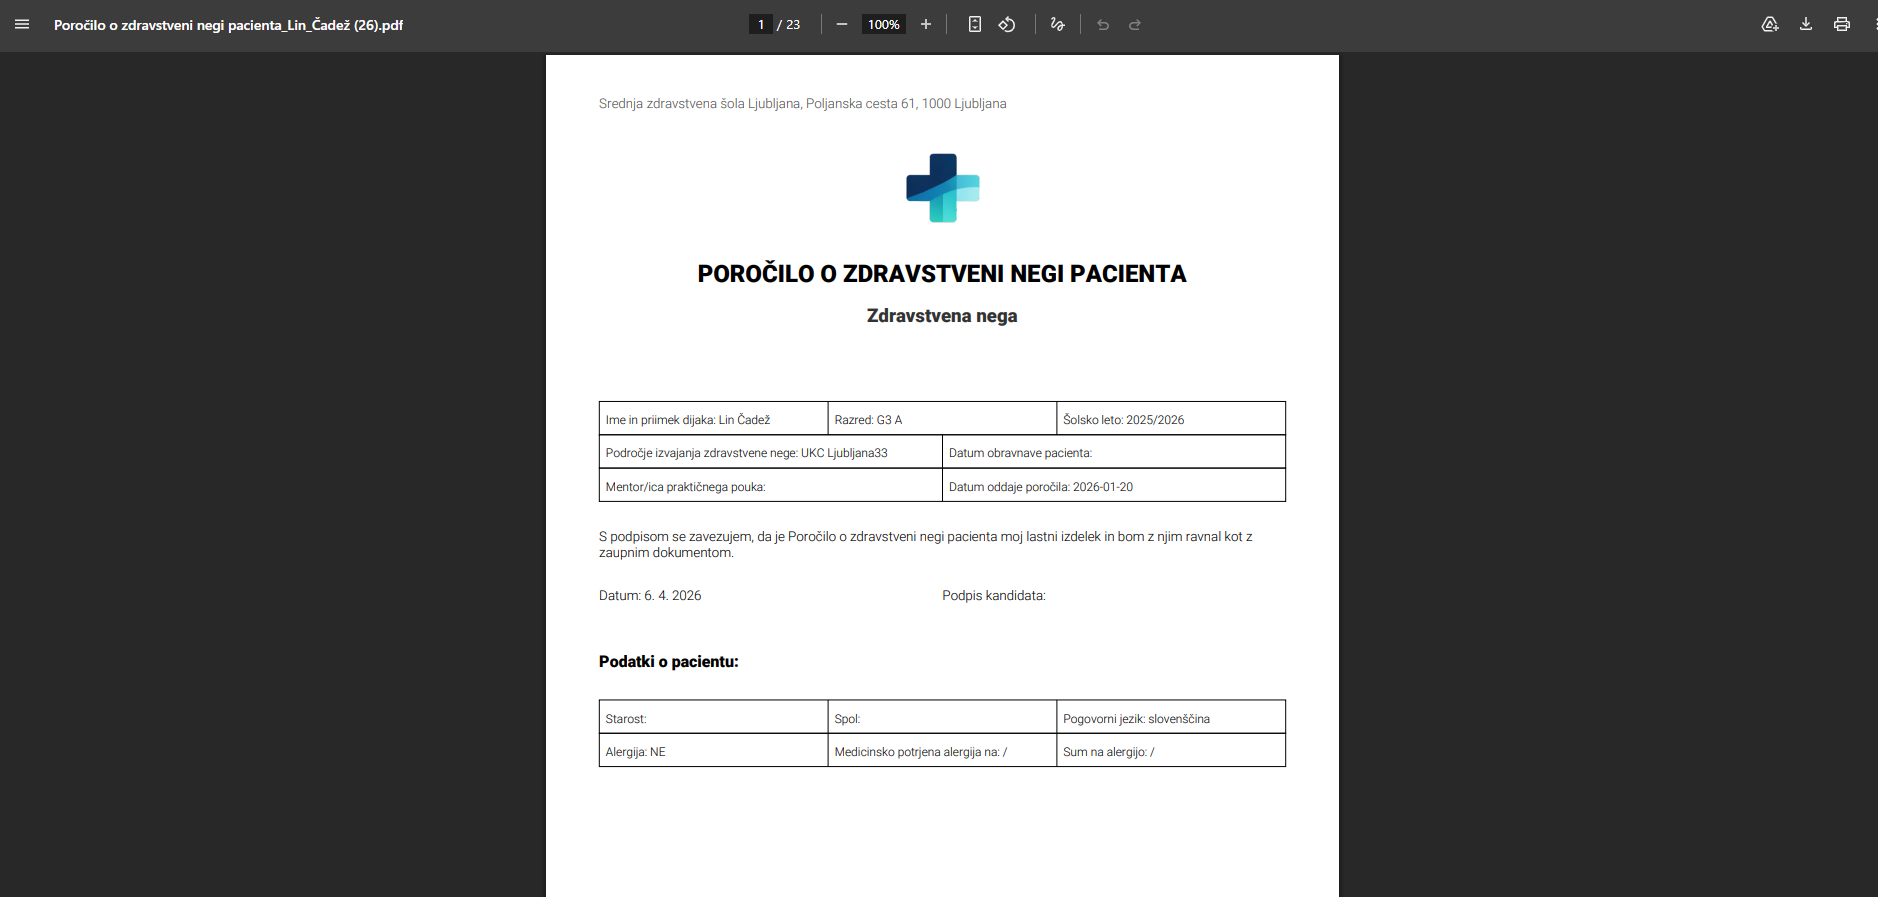
\includegraphics[width=0.8\textwidth]{slike/Pdf_primer_generira_za_izmislejno_osebo.png}
    \caption{Slika 5: Primer izvoza poročila v PDF}
\end{figure}

\section{Zaključek}

Razvoj aplikacije MediForm mi je pokazal, da je mogoče z ustreznim načrtovanjem in dobrim sodelovanjem z naročnikom razviti uporabno digitalno rešitev za šolsko okolje. Aplikacija je nastala zato, ker sem želel odpraviti težave, ki so se pojavljale pri ročnem izpolnjevanju poročil o praktičnem pouku.

Ugotovil sem, da je bila najpomembnejša dobra komunikacija s stranko. Sproti sem preverjal, kaj naročnica res potrebuje, in na podlagi njenih pripomb popravljal aplikacijo. To se je izkazalo za pravilno odločitev, saj so bile funkcionalnosti bolj usmerjene v resnične potrebe uporabnikov.

Pri tehnični izvedbi sem se srečal z več izzivi, predvsem pri organizaciji obrazcev, samodejnem shranjevanju podatkov in pripravi izvoza v PDF. Vsak problem sem reševal po korakih in sproti preverjal skupaj z naročnico, zato je bila končna rešitev stabilna in uporabna v praksi.

Na koncu sem ugotovil, da MediForm uporabnikom olajša delo, zmanjšuje ročno pisanje in omogoča bolj sprotno izpolnjevanje dokumentacije. Zato menim, da je digitalizacija tovrstnih postopkov smiselna in koristna rešitev za izobraževalno okolje.

\newpage

\section*{Viri}

European Commission. (2020). \textit{Digital Education Action Plan 2021--2027}. European Commission.

Firebase. (2026). \textit{Firebase Documentation}. Dostopno prek: \url{https://firebase.google.com/docs/}

Redecker, C. (2017). \textit{European Framework for the Digital Competence of Educators (DigCompEdu)}. European Commission.

Selwyn, N. (2016). \textit{Should robots replace teachers? AI and the future of education}. Polity Press.

React. (2026). \textit{React Documentation}. Dostopno prek: \url{https://react.dev/}

Express.js. (2026). \textit{Express.js Documentation}. Dostopno prek: \url{https://expressjs.com/}

\newpage

\section*{Priloge}

\subsection*{Priloga A: Spletno mesto in GitHub}

Spletna aplikacija MediForm je dostopna na naslovu: \url{https://mediform.cadez.eu/}

Izvorna koda projekta je dostopna na GitHubu:
\begin{itemize}
    \item \url{https://mediform.cadez.eu/}
    \item \url{https://github.com/lin-cadez/MediForm}
\end{itemize}

\subsection*{Priloga B: Tehnične specifikacije}

\begin{itemize}
    \item Frontend: React, TypeScript, Tailwind CSS, Vite
    \item Shranjevanje: cookies in localStorage
    \item Objava: statično gostovanje
\end{itemize}

\newpage

\section*{Izjava o avtorstvu}

Izjavljam, da je strokovno poročilo \textit{Spletna aplikacija MediForm za digitalno poročanje o zdravstveni negi} v celoti moje avtorsko delo, ki sem ga izdelal/-a samostojno s pomočjo navedene literature in pod vodstvom mentorja.

\vspace{1.5cm}

Ljubljana, april 2026 \hfill Lin Čadež

\end{document}
